\documentclass{beamer}

\usepackage{graphicx}
\usepackage{caption}

\begin{document}
	
	\begin{frame}[plain]
		\begin{figure}
			\centering
			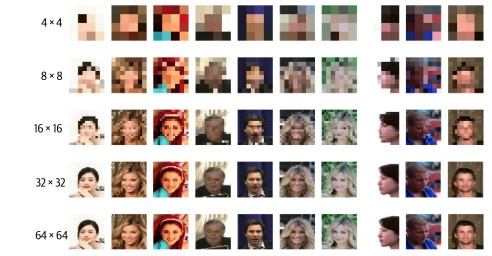
\includegraphics[width=\textwidth,height=0.85\textheight,keepaspectratio]{101.jpg}
			\caption{Images in the dataset can be compressed to lower resolution using
				interpolation}
		\end{figure}
	\end{frame}
	
	\begin{frame}[plain]
		\begin{figure}
			\centering
			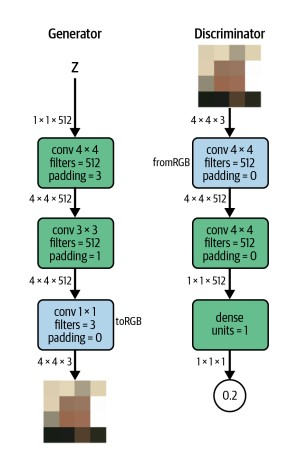
\includegraphics[width=\textwidth,height=0.85\textheight,keepaspectratio]{102.jpg}
			\caption{The generator and discriminator architectures for the first stage of the Pro‐GAN training process}
		\end{figure}
	\end{frame}
	
	\begin{frame}[plain]
		\begin{figure}
			\centering
			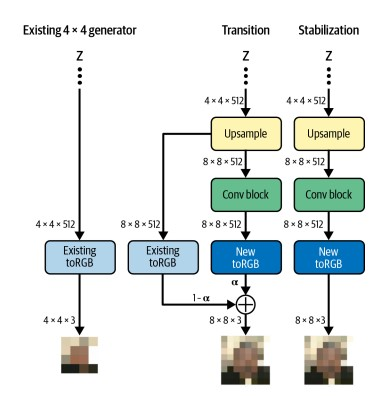
\includegraphics[width=\textwidth,height=0.78\textheight,keepaspectratio]{103.jpg}
			\caption{The ProGAN generator training process, expanding the network from 4 × 4
				images to 8 × 8 (dotted lines represent the rest of the network, not shown)}
		\end{figure}
	\end{frame}
	
	\begin{frame}[plain]
		\begin{figure}
			\centering
			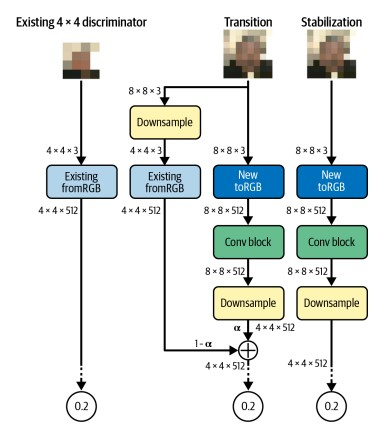
\includegraphics[width=\textwidth,height=0.78\textheight,keepaspectratio]{104.jpg}
			\caption{The ProGAN discriminator training process, expanding the network from
				4 × 4 images to 8 × 8 (dotted lines represent the rest of the network, not shown)}
		\end{figure}
	\end{frame}
	
	\begin{frame}[plain]
		\begin{figure}
			\centering
			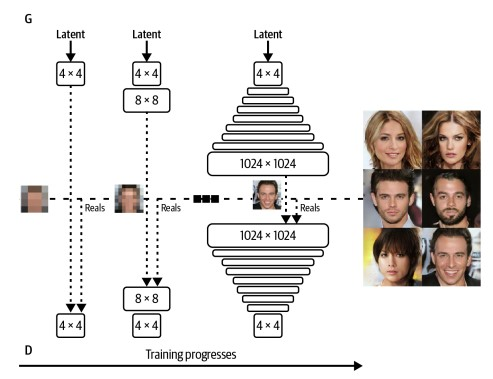
\includegraphics[width=\textwidth,height=0.8\textheight,keepaspectratio]{105.jpg}
			\caption{The ProGAN training mechanism, and some example generated faces}
		\end{figure}
	\end{frame}
	
	\begin{frame}[plain]
		\begin{figure}
			\centering
			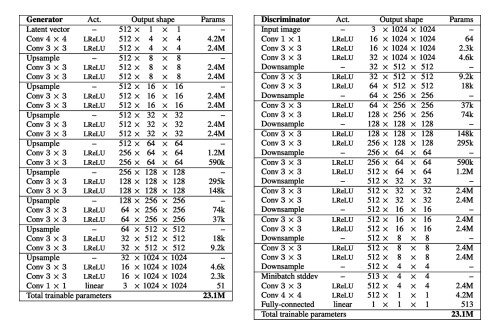
\includegraphics[width=\textwidth,height=0.85\textheight,keepaspectratio]{106.jpg}
			\caption{The ProGAN generator and discriminator used to generate 1,024 × 1,024 – pixel CelebA faces}
		\end{figure}
	\end{frame}
	
	\begin{frame}[plain]
		\begin{figure}
			\centering
			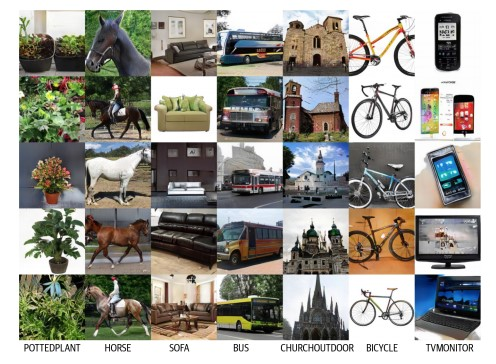
\includegraphics[width=\textwidth,height=0.85\textheight,keepaspectratio]{107.jpg}
			\caption{Generated examples from a ProGAN trained progressively on the LSUN
				dataset at 256 × 256 resolution}
		\end{figure}
	\end{frame}
	
	\begin{frame}[plain]
		\begin{figure}
			\centering
			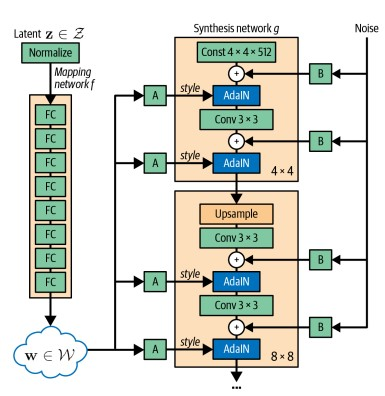
\includegraphics[width=\textwidth,height=0.85\textheight,keepaspectratio]{108.jpg}
			\caption{The StyleGAN generator architecture}
		\end{figure}
	\end{frame}
	
	\begin{frame}[plain]
		\begin{figure}
			\centering
			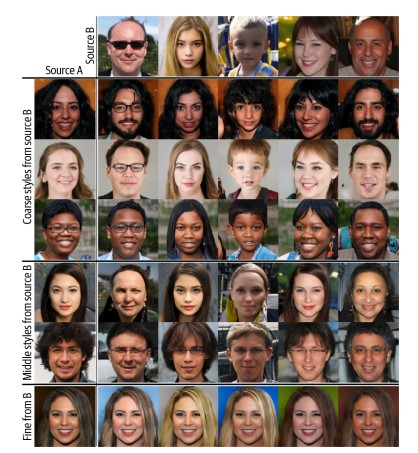
\includegraphics[width=\textwidth,height=0.85\textheight,keepaspectratio]{109.jpg}
			\caption{Merging styles between two generated images at different levels of detail}
		\end{figure}
	\end{frame}
	
	\begin{frame}[plain]
		\begin{figure}
			\centering
			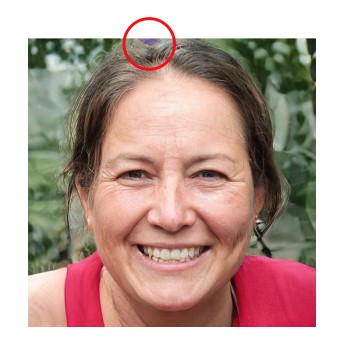
\includegraphics[width=\textwidth,height=0.78\textheight,keepaspectratio]{1010.jpg}
			\caption{ An artifact in a StyleGAN-generated image of a face}
		\end{figure}
	\end{frame}
	
	\begin{frame}[plain]
		\begin{figure}
			\centering
			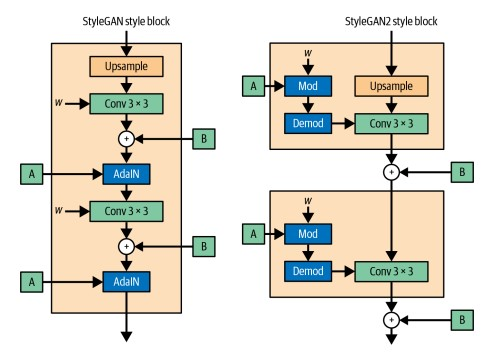
\includegraphics[width=\textwidth,height=0.8\textheight,keepaspectratio]{1011.jpg}
			\caption{A comparison between the StyleGAN and StyleGAN2 style blocks}
		\end{figure}
	\end{frame}
	
	\begin{frame}[plain]
		\begin{figure}
			\centering
			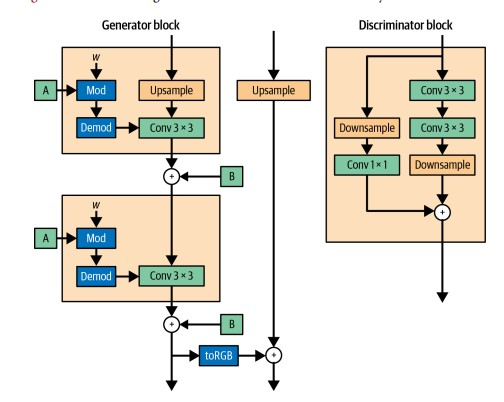
\includegraphics[width=\textwidth,height=0.85\textheight,keepaspectratio]{1012.jpg}
			\caption{The generator and discriminator blocks in StyleGAN2}
		\end{figure}
	\end{frame}
	
	\begin{frame}[plain]
		\begin{figure}
			\centering
			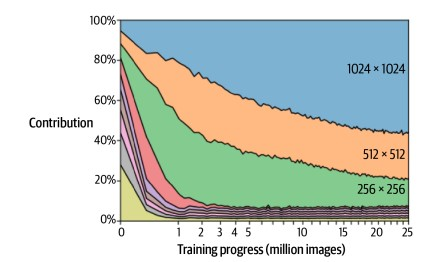
\includegraphics[width=\textwidth,height=0.78\textheight,keepaspectratio]{1013.jpg}
			\caption{The contribution of each resolution layer to the output of the generator, by
				training time}
		\end{figure}
	\end{frame}
	
	\begin{frame}[plain]
		\begin{figure}
			\centering
			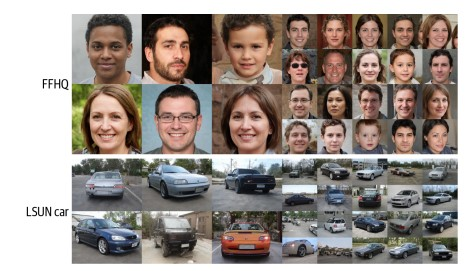
\includegraphics[width=\textwidth,height=0.78\textheight,keepaspectratio]{1014.jpg}
			\caption{Uncurated StyleGAN2 output for the FFHQ face dataset and LSUN car
				dataset}
		\end{figure}
	\end{frame}
	\begin{frame}[plain]
		\begin{figure}
			\centering
			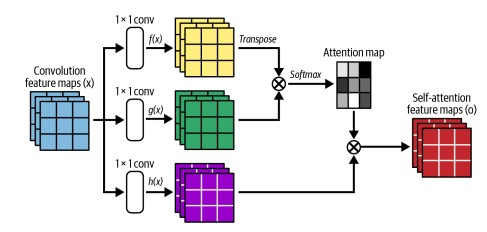
\includegraphics[width=\textwidth,height=0.78\textheight,keepaspectratio]{1015.jpg}
			\caption{The self-attention mechanism within the SAGAN model}
		\end{figure}
	\end{frame}
	\begin{frame}[plain]
		\begin{figure}
			\centering
			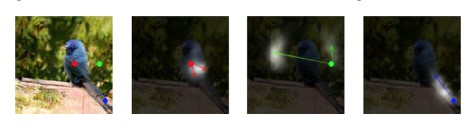
\includegraphics[width=\textwidth,height=0.78\textheight,keepaspectratio]{1016.jpg}
			\caption{A SAGAN-generated image of a bird (leftmost cell) and the attention
				maps of the final attention-based generator layer for the pixels covered by the three col‐
				ored dots (rightmost cells)}
		\end{figure}
	\end{frame}
	
	\begin{frame}[plain]
		\begin{figure}
			\centering
			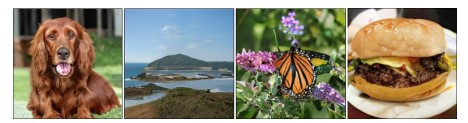
\includegraphics[width=\textwidth,height=0.78\textheight,keepaspectratio]{1017.jpg}
			\caption{Examples of images generated by BigGAN}
		\end{figure}
	\end{frame}
	
	\begin{frame}[plain]
		\begin{figure}
			\centering
			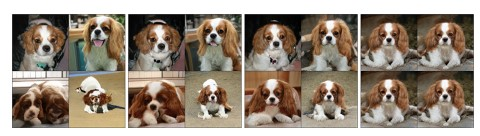
\includegraphics[width=\textwidth,height=0.78\textheight,keepaspectratio]{1018.jpg}
			\caption{The truncation trick: from left to right, the threshold is set to 2, 1, 0.5, and
				0.04}
		\end{figure}
	\end{frame}
	
	\begin{frame}[plain]
		\begin{figure}
			\centering
			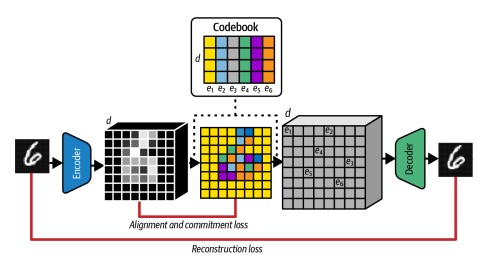
\includegraphics[width=\textwidth,height=0.78\textheight,keepaspectratio]{1019.jpg}
			\caption{A diagram of a VQ-VAE}
		\end{figure}
	\end{frame}
	
	\begin{frame}[plain]
		\begin{figure}
			\centering
			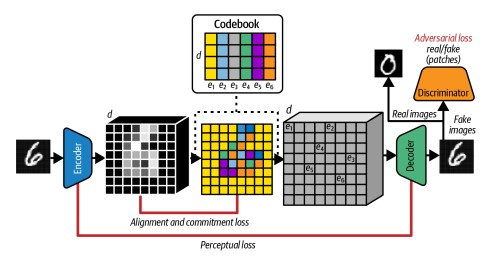
\includegraphics[width=\textwidth,height=0.78\textheight,keepaspectratio]{1020.jpg}
			\caption{A diagram of a VQ-GAN: the GAN discriminator helps to encourage the
				VAE to generate less blurry images through an additional adversarial loss term}
		\end{figure}
	\end{frame}
	
		\begin{frame}[plain]
		\begin{figure}
			\centering
			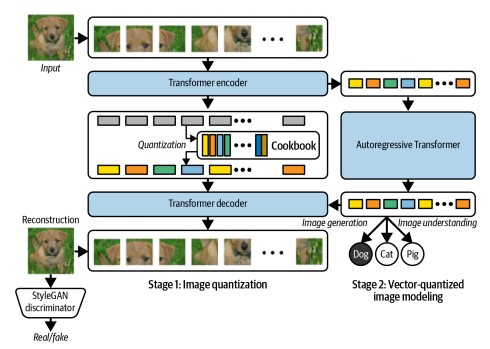
\includegraphics[width=\textwidth,height=0.78\textheight,keepaspectratio]{1021.jpg}
			\caption{A diagram of a ViT VQ-GAN: the GAN discriminator helps to encourage
				the VAE to generate less blurry images through an additional adversarial loss term}
		\end{figure}
	\end{frame}
		\begin{frame}[plain]
		\begin{figure}
			\centering
			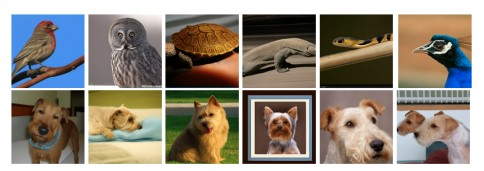
\includegraphics[width=\textwidth,height=0.78\textheight,keepaspectratio]{1022.jpg}
			\caption{Example images generated by a ViT VQ-GAN trained on ImageNet}
		\end{figure}
	\end{frame}
	
\end{document}